\section{Writing}

\lettrine{T}{his} section outlines advice, tips, and suggestions to consider when writing. 
The writing instruction provided is in no way conclusive, however, it is the author's hope that it will be developed through time to ease students into the expectations of academic writing. 

\subsection{Document Setup}

The most important thing to consider before even beginning to write is what are the expectations? 
Every technical writing conference/journal/thesis will have a set of formatting requirements \cite{writingAIAA,writingThesisUofC}. 
Review these requirements \textbf{before} writing to save time later re-formatting everything that was incorrect initially. 
These organizational formatting requirements are the be-all-end-all to discussions about formatting, the document must align. 

\subsubsection{Figures and Tables}

General rules exist that apply to both figures and tables. A couple of these shared rules are listed: 
\begin{itemize}
	\item Figures and tables must always be introduced in-text before they are presented, 
	\item Figures and tables should not have titles, 
	\item Figure and table text should match document size and font, 
	\item Captions should remain within the margins of the figure/table they describe, 
	\item Captions should end with a period (as they are a proper sentence).
\end{itemize}

\noindent
Specific figure considerations include: 
\begin{itemize}
	\item Colour should be chosen in such a way that data will still be differentiable in greyscale,
	\item Gradient colour should start/end light/dark, not have white in the middle of the gradient as this could become confusing in greyscale, an example of gradients is presented in \cref{fig:gradientExample},
	\item Ideally, different data marks should be utilized to ensure data is differentiable in greyscale, 
	\item Colour choice should be considerate of colourblind people \cite{colourScienceMisuse},
	\item Axes should end on definitive numbers. 
\end{itemize}

\noindent
Examples of these aforementioned rules are presented in \cref{fig:gradientExample} and \ref{fig:dataExample}. 


\begin{figure}[hbt!]
	\centering
	\captionsetup{width=\textwidth}
	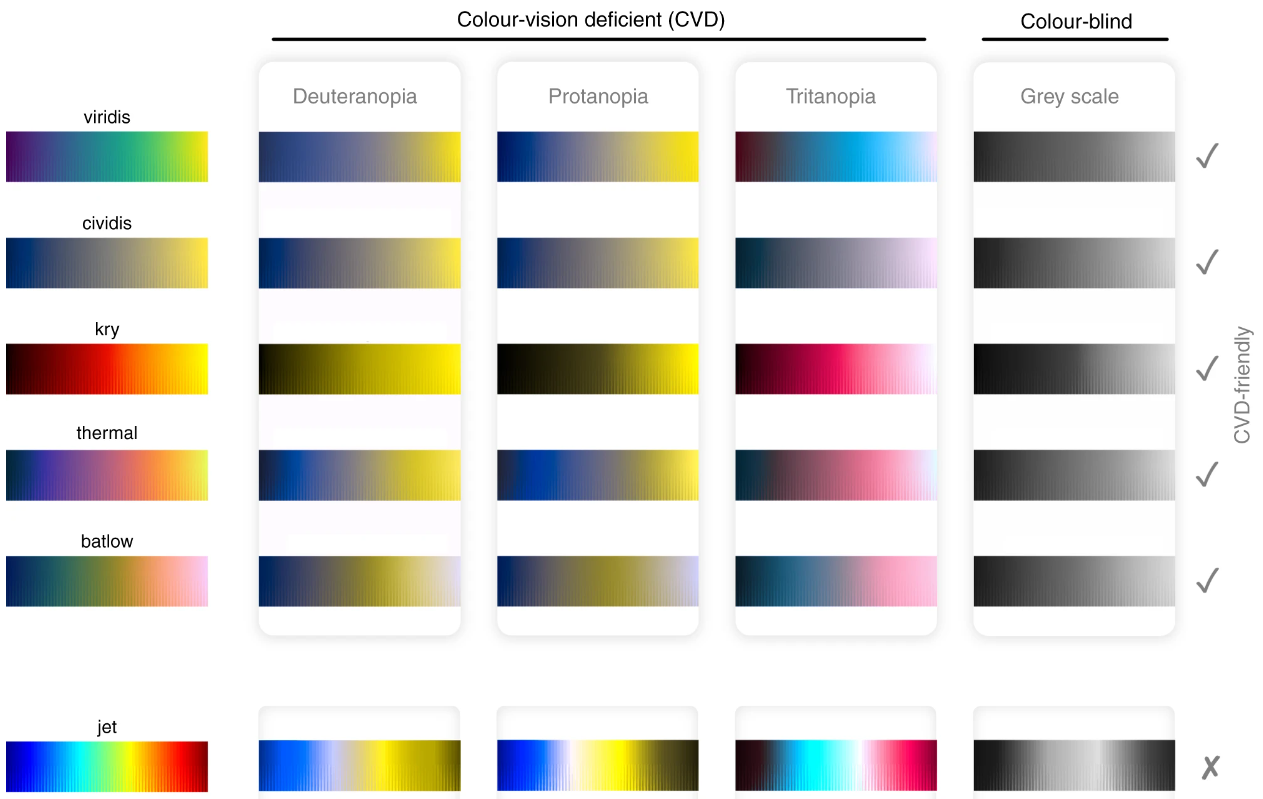
\includegraphics[width=\textwidth]{Photos/Figures/gradients.png}
	\caption{How common gradients appear to various colourblind diagnoses, adapted from \citeauthor{colourScienceMisuse} \cite{colourScienceMisuse}.}
	\label{fig:gradientExample}
	\hfill
\end{figure}



\begin{figure}[hbt!]
	\centering
	\captionsetup{width=0.5\textwidth}
	\def\svgwidth{0.55\textwidth}
	\input{Photos/Figures/MUFASAandGoJettandTranceRelationshipComparison-InverseTimeConstant-MachNumber-2column_Editted.eps_tex}
	\caption{MUFASA B aerodynamic design and coordinate system. Notice how different symbols and colours are used. Also note how the ends of the x and y axes are denoted by a number and not left ambiguously floating.}
	\label{fig:dataExample}
	\hfill
\end{figure}


\subsection{General Writing}

Common writing mistakes and misconceptions are presented in this section. It is the authors hope this list is useful, not to mention also not containing errors of its own. 
Great resources are found online \cite{writingAIAA}, and at the University of Calgary \cite{writingUofC,writingCoursesUofC}. 


\subsubsection{Language}

A conference/journal/thesis requires exact language be used. 
Using words such as \textit{can}, \textit{could}, and \textit{would} make the document sound uncertain. 
This type of uncertain wording should only be used when discussing potential future work, which is always inherently uncertain. 
Do not write "\textit{...this can be seen in Fig...,}", instead write "\textit{...this is presented in Fig...}".

A word on the use of the word \textit{this}. 
The word \textit{this} should not start a sentence unless it is followed directly with an indication of what \textit{this} is. 
A sentence should be a standalone idea, thus, without reiterating to the reader what \textit{this} is, it is very easy for the reader to become confused. 
Parallel to this concept of the uncertainty of \textit{this} is how authors sometimes use \textit{it} without explaining what \textit{it} is they are referring to. 

Word choice is paramount and matters. While often used interchangeably in normal language, \textit{compute}, \textit{evaluate}, and \textit{calculate} suggest very different approaches were taken. 


\subsubsection{Commas}

Always use the Oxford comma when making a list. The Oxford comma helps the reader understand if the last two items in a list are together or separate. 

\subsection{Referencing}
Referencing is a vital part of science, a way to track that all scientific statements are supported by evidence \cite{referncingVirtues}. 